\documentclass[12pt]{article}
\usepackage{array,booktabs}
\usepackage{graphicx} % Required for inserting images
\usepackage{setspace}
\usepackage[margin=2.5cm]{geometry} % margins
\usepackage[parfill]{parskip}
\usepackage{enumitem}
\usepackage{amsfonts,latexsym,amsthm,amssymb,amsmath,amscd,euscript}

%Chemistry Packages
\usepackage{chemfig}
\usepackage{mhchem}
\usepackage{chemformula}
\usepackage{siunitx}
\sisetup{group-digits=false}
\usepackage{cancel}

\usepackage{pgfplots}
\pgfplotsset{compat=1.18}

\setlength{\parindent}{0pt}
\AtBeginDocument{\setstretch{1.125}}

\title{Enzyme Lab}
\author{Anthony Yu}
\date{October 2024}

\begin{document}

%Some new commands
\newcommand{\problem}[1]{\subsection*{Problem {#1}}}
\newenvironment{enumAlph}{\begin{enumerate}[label=(\alph*)]}{\end{enumerate}}

\makeatletter
\newcommand{\skipitems}[1]{%
\addtocounter{\@enumctr}{#1}%
}
\makeatother

\newcommand{\chunit}[3]{\qty{#1}{{#2}\,\ce{#3}}}
\newcommand{\chuniteval}[3]{\qty[evaluate-expression]{#1}{{#2}\,\ce{#3}}}

\newtheorem{definition}{Definition}

\maketitle

\section*{Data}
\subsection*{Procedure A}
\begin{table}[h]
    \centering
    \begin{tabular}{cccccccccc}
        \toprule
        Time (s) & 0 & 15 & 30 & 45 & 60 & 75 & 90 & 105 & 120 \\
        \midrule
        \ch{H2O2}/\ch{H2O} & 24.2 & 21.6 & 20.5 & 20.4 & 20.3 & 20.3 & 20.1 & 20.1 & 20.1 \\
        \ch{H2O2}/lj & 23.5 & 29.1 & 29.9 & 29.3 & 29 & 29 & 28.8 & 28.2 & 28.2 \\
        \bottomrule
    \end{tabular}
    \caption{Table of Measurements over Time for Procedure A and Procedure B}
    \label{tab:measurements}
\end{table}
\begin{figure}[h]
    \centering
    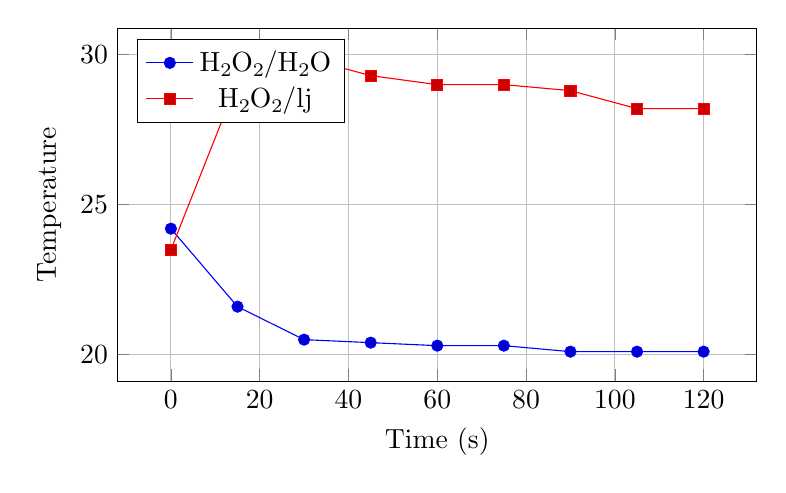
\begin{tikzpicture}
        \begin{axis}[
            xlabel={Time (s)},
            ylabel={Temperature},
            legend pos=north west,
            grid=major,
            width=0.8\textwidth,
            height=0.5\textwidth
        ]
        \addplot coordinates {(0,24.2) (15,21.6) (30,20.5) (45,20.4) (60,20.3) (75,20.3) (90,20.1) (105,20.1) (120,20.1)};
        \addlegendentry{\ch{H2O2}/\ch{H2O}}

        \addplot coordinates {(0,23.5) (15,29.1) (30,29.9) (45,29.3) (60,29) (75,29) (90,28.8) (105,28.2) (120,28.2)};
        \addlegendentry{\ch{H2O2}/lj}
        \end{axis}
    \end{tikzpicture}
    \caption{Graph of Measurements over Time for Procedure A and Procedure B}
    \label{fig:measurements}
\end{figure}

\newpage

\subsection*{Procedure B}
\begin{table}[h]
    \centering
    \begin{tabular}{cccccccccc}
        \toprule
        Time (s) & 0 & 15 & 30 & 45 & 60 & 75 & 90 & 105 & 120 \\ 
         \midrule
         \ch{H2O2}/boiled lj & 22 & 20.5 & 20.1 & 20.1 & 20 & 20.2 & 20.2 & 20.1 & 20.2 \\ 
         \ch{H2O2}/acid lj & 22 & 21.5 & 21.5 & 21 & 21 & 21 & 21.1 & 21 & 20.9 \\ 
         \ch{H2O2}/base lj & 22 & 21.2 & 21.2 & 21.3 & 21.2 & 21.5 & 21.6 & 21.8 & 21.9 \\ 
         \ch{H2O2}/salt lj & 23 & 23.2 & 24.5 & 26.9 & 28.9 & 31 & 31.5 & 31.9 & 31.7 \\ 
         Boiled \ch{H2O2}/lj & 23 & 31 & 38 & 41 & 41 & 41 & 39 & 38 & 37.5 \\ 
         \bottomrule
    \end{tabular}
    \caption{Table of Measurements over Time for Procedure B}
    \label{tab:measurements_b}
\end{table}
\begin{figure}[h]
    \centering
    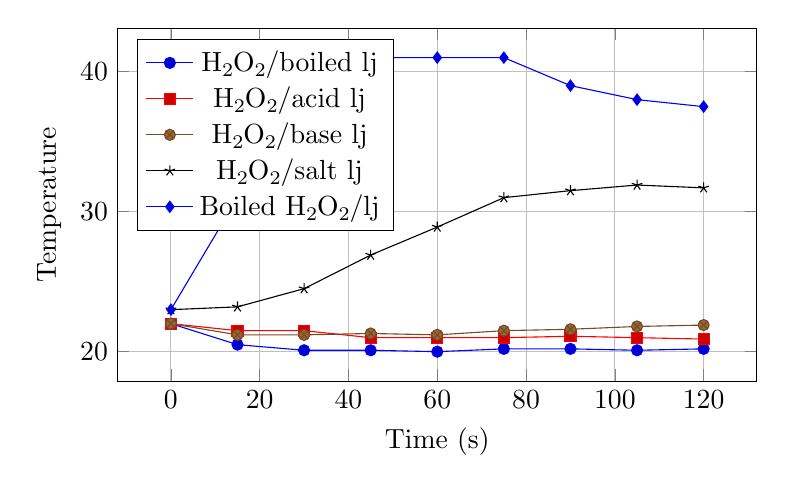
\begin{tikzpicture}
        \begin{axis}[
            xlabel={Time (s)},
            ylabel={Temperature},
            legend pos=north west,
            grid=major,
            width=0.8\textwidth,
            height=0.5\textwidth
        ]
        \addplot coordinates {(0,22) (15,20.5) (30,20.1) (45,20.1) (60,20) (75,20.2) (90,20.2) (105,20.1) (120,20.2)};
        \addlegendentry{\ch{H2O2}/boiled lj}

        \addplot coordinates {(0,22) (15,21.5) (30,21.5) (45,21) (60,21) (75,21) (90,21.1) (105,21) (120,20.9)};
        \addlegendentry{\ch{H2O2}/acid lj}

        \addplot coordinates {(0,22) (15,21.2) (30,21.2) (45,21.3) (60,21.2) (75,21.5) (90,21.6) (105,21.8) (120,21.9)};
        \addlegendentry{\ch{H2O2}/base lj}

        \addplot coordinates {(0,23) (15,23.2) (30,24.5) (45,26.9) (60,28.9) (75,31) (90,31.5) (105,31.9) (120,31.7)};
        \addlegendentry{\ch{H2O2}/salt lj}

        \addplot coordinates {(0,23) (15,31) (30,38) (45,41) (60,41) (75,41) (90,39) (105,38) (120,37.5)};
        \addlegendentry{Boiled \ch{H2O2}/lj}
        \end{axis}
    \end{tikzpicture}
    \caption{Graph of Measurements over Time for Procedure B}
    \label{fig:measurements_b}
\end{figure}

\newpage


\subsection*{Procedure C}
\begin{table}[h]
    \centering
    \begin{tabular}{cccccccccc}
        \toprule
        Time (s) & 0 & 15 & 30 & 45 & 60 & 75 & 90 & 105 & 120 \\ 
        \midrule
        1.5\% \ch{H2O2} & 22 & 26.1 & 26.9 & 28.9 & 26.5 & 26.2 & 26.2 & 26.1 & 26 \\ 
        3\% \ch{H2O2} & 23 & 29.1 & 30 & 29.9 & 29.1 & 29 & 28.9 & 28.5 & 28.2 \\ 
        6\% \ch{H2O2} & 23 & 34 & 37 & 36.5 & 36 & 35.1 & 34.9 & 34.1 & 33.9 \\ 
        10\% \ch{H2O2} & 23 & 38 & 43 & 42 & 41 & 40 & 39 & 38 & 37.5 \\ 
        \bottomrule
    \end{tabular}
    \caption{Table of Measurements over Time for Procedure C}
    \label{tab:measurements_c}
\end{table}
\begin{figure}[h]
    \centering
    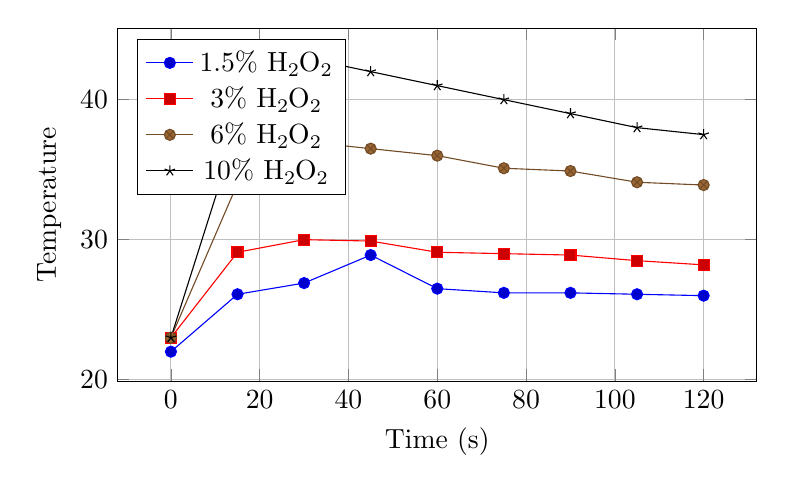
\begin{tikzpicture}
        \begin{axis}[
            xlabel={Time (s)},
            ylabel={Temperature},
            legend pos=north west,
            grid=major,
            width=0.8\textwidth,
            height=0.5\textwidth
        ]
        \addplot coordinates {(0,22) (15,26.1) (30,26.9) (45,28.9) (60,26.5) (75,26.2) (90,26.2) (105,26.1) (120,26)};
        \addlegendentry{1.5\% \ch{H2O2}}

        \addplot coordinates {(0,23) (15,29.1) (30,30) (45,29.9) (60,29.1) (75,29) (90,28.9) (105,28.5) (120,28.2)};
        \addlegendentry{3\% \ch{H2O2}}

        \addplot coordinates {(0,23) (15,34) (30,37) (45,36.5) (60,36) (75,35.1) (90,34.9) (105,34.1) (120,33.9)};
        \addlegendentry{6\% \ch{H2O2}}

        \addplot coordinates {(0,23) (15,38) (30,43) (45,42) (60,41) (75,40) (90,39) (105,38) (120,37.5)};
        \addlegendentry{10\% \ch{H2O2}}
        \end{axis}
    \end{tikzpicture}
    \caption{Graph of Measurements over Time for Procedure C}
    \label{fig:measurements_c}
\end{figure}


\section*{Data Analysis}

\subsection*{Question 2}
\begin{enumAlph}
    \item The test tube with water and \ch{H2O2} saw a slight decrease in temperature
    because the water was stored colder than room temperature. This test tube serves as a control. It is to show
    the speed of reaction and temperature increases without enzymes, 
    confirming that the temperature increase we saw
    was due to the liver juice catalyzing the decomposition of \ch{H2O2}. 
    \item We could tell a reaction was occuring in test tube B 
    because the temperature increased, as shown by the thermometer.
    Additionally, bubbles comprised of oxygen gas were quickly released, overfilling
    the test tube. This means that some liquid has transformed into gas. 
    \item Before we added the enzyme, the reaction was occuring at 
    an extremely slow rate. I could tell because when water was added to H2O2, 
    the temperature did not increase. According to Mr. 
    Chisholm, if a sealed bottle of hydrogen peroxide was left alone,
    it would take years for it to decompose.
    \item When we added the enzyme, the
    reaction rate increased significantly, as indicated by the temperature increase of the solution from 
    23.5 degrees Celsius to 29.1 degrees Celsius in 15 seconds. Additionally, the reaction seemed to have
    subsided after 30 seconds, when the temperature reached its peak of 29.9 degrees Celsius, and then
    slowly decreased. Mr. Chisholm stated in class that catalase is the fastest
    enzyme in the body. 
    \item Catalase speeds up the reaction through the induced fit model. 
    The substrate, hydrogen peroxide, fits into the enzyme's active site, 
    matching its shape, size, and charge. The R groups of the amino acids in catalase’s active site are polar, which helps attract and stabilize the substrate during binding.
    
    This causes the enzyme to change 
    shape slightly, putting stress on the bonds in the hydrogen peroxide 
    molecule, making them unstable and lowering the activation energy 
    required for the reaction, as shown in the energy hill diagram below. The bonds break, producing water and oxygen. 
    Once these products are formed, they no longer fit the active site, 
    so they are released, and the enzyme is free to catalyze another reaction.

    \begin{center}
    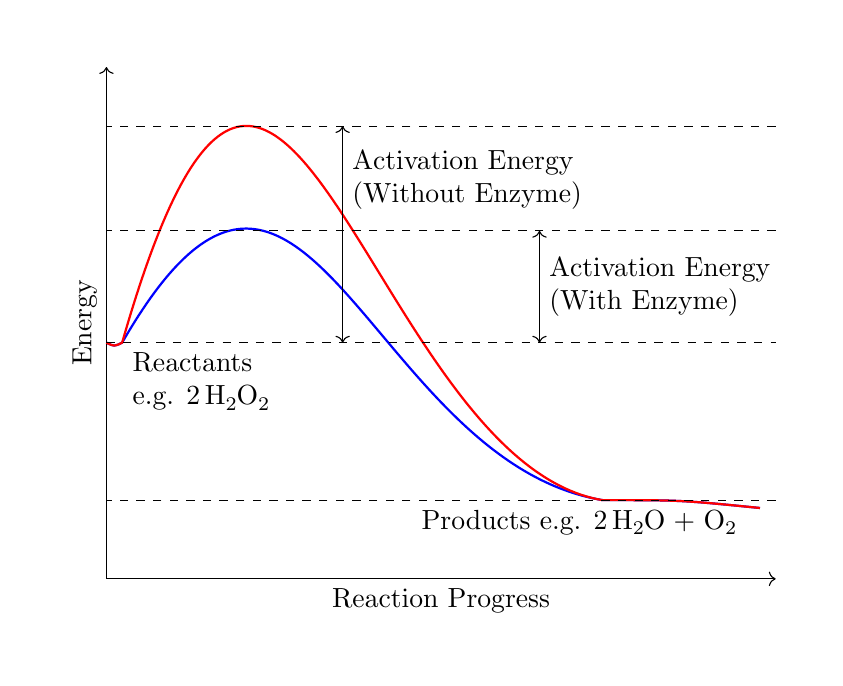
\begin{tikzpicture}

        \clip (-1,-1) rectangle (9, 7);
        
        % Axes
        \draw[->] (0,0) -- (8.5,0) node[midway, below] {Reaction Progress};
        \draw[->] (0,0) -- (0,6.5) node[midway, above, rotate=90] {Energy};
    
        % Reaction curve
        \draw[thick, blue] (0,3) .. controls (0.1,2.95) .. (0.2,3) .. controls (2.5,7) and (3.3,1.5) .. (6.3,1) .. controls (7.3,1) .. (8.3,0.9);
        \draw[thick, red] (0,3) .. controls (0.1,2.95) .. (0.2,3) .. controls (2.2,10) and (3.3,1.5) .. (6.3,1) .. controls (7.3,1) .. (8.3,0.9);
    
        % Labels
        \node at (1.2,3) [below, align=left] {Reactants \\e.g. \ch{2 H2O2}};
        \node at (6,1) [below] {Products e.g. \ch{2 H2O + O2}};
        \draw[dashed] (0,3) -- (8.5,3);
        \draw[dashed] (8.5,1) -- (0,1);
        \draw[dashed] (8.5,4.42) -- (0,4.42);
        \draw[dashed] (8.5,5.75) -- (0,5.75);

        % Activation energy label for Without Enzyme
        \draw[<->] (3,3) -- (3,5.75) node[pos=0.75,right, align=left] {Activation Energy\\(Without Enzyme)};
        
        % Activation energy label for With Enzyme
        \draw[<->] (5.5,3) -- (5.5,4.42) node[midway,right, align=left] {Activation Energy\\(With Enzyme)};
        
    \end{tikzpicture}
    \end{center}

    \item When the \ch{H2O2} bonds are broken, more stable water and oxygen gas molecules
    are reformed. This results in an overall exothermic reaction, which explains where
    the heat energy came from. 
    \item The gas was oxygen. We showed that as 
    Mr. Chisholm brought .  
    \item The formula for the reaction is:
    \begin{center}
        \ch{2 H2O2 -> 2 H2O + O2}
    \end{center}
    The products are not very harmful to cells. Water is a universal solvent, and facilitates
    many reactions necessary for life, such as hydrolysis. Oxygen is neccesary 
    for cellular respiration, which is the process that generates ATP. Hence,
    the liver is a very important organ in the body, as it metabolizes drugs and waste
    products into molecules that can be utilized by the body. 

    \item The reaction is advantageous in peroxisomes is because they provide
    the optimal environment for the enzymes that 
    facilitate the decomposition of hydrogen peroxide. Additionally, peroxisomes isolate 
    the inside from the rest of the cell. There, hydrogen peroxide is
    made and instantly broken down in the peroxisome, so it does not have a chance to
    damage the cell.

\end{enumAlph}

\subsection*{Question 3}
\begin{enumAlph}
    \item 
    
    \begin{enumerate}[label=\arabic*.]
        \item Boiled liver juice: Enzymes, when subjected to 
        high temperatures, undergo denaturation, which is
        when they lose their shape and function. This is because heat increases the kinetic energy of molecules
        causing them to vibrate more, which disrupts the hydrogen bonds that
        hold the protein in shape. Even when the temperature lowers back down, 
        the shape will not return to normal. Catalase enzymes stop working properly at
        around 40 degrees Celsius, so boiling them at 100 degrees will completely
        destroy their function. This is reflected in our data, indicating no 
        temperature increase at all. 
        
        \item Liver juice in acid: Similarly, most enzymes denature under
        a low pH environment, as the abundance of \ch{H+} ions can disrupt
        the hydrogen bonds in the amino acids. This explains why barely any reaction
        occured. 

        \item Liver juice in base: Most enzymes also denature under
        a high pH environment, as the abundance of \ch{OH-} ions can disrupt
        the hydrogen bonds in the amino acids. This explains why barely any reaction
        occured. 

        \item Liver juice in salt: The 15 percent salt solution was not enough to denature the 
        enzymes. Although it did slow down the reaction, the reaction proceeded 
        as normal. This is an interesting result. 

        \item Liver juice with boiled \ch{H2O2}: The boiled \ch{H2O2} reacted faster because 
        some water molecules in the aqueous solution are removed when boiled, while 
        \ch{H2O2} stays intact, thus
        increasing the overall concentration of \ch{H2O2}. Enzymes work better when 
        there is a higher concentration of substrate, as they are more likely to collide
        with the active site.

        
    \end{enumerate}
\end{enumAlph}



\end{document}



\section*{Data Analysis}

\subsection*{Question 2}
\begin{enumAlph}
    \item 
\end{enumAlph}

\end{document}